	\documentclass[10pt,oneside]{CBFT_book}
	% Algunos paquetes
	\usepackage{amssymb}
	\usepackage{amsmath}
	\usepackage{graphicx}
	\usepackage{libertine}
	\usepackage[bold-style=TeX]{unicode-math}
	\usepackage{lipsum}

	\usepackage{natbib}
	\setcitestyle{square}

	\usepackage{polyglossia}
	\setdefaultlanguage{spanish}


	\usepackage{CBFT.estilo} % Cargo la hoja de estilo

	% Tipografías
	% \setromanfont[Mapping=tex-text]{Linux Libertine O}
	% \setsansfont[Mapping=tex-text]{DejaVu Sans}
	% \setmonofont[Mapping=tex-text]{DejaVu Sans Mono}

	%===================================================================
	%	DOCUMENTO PROPIAMENTE DICHO
	%===================================================================

\begin{document}

% =================================================================================================
\chapter{Fenómenos dependientes del tiempo}
% =================================================================================================




% =================================================================================================
\section{Medios magnéticos}
% =================================================================================================

\begin{figure}[htb]
	\begin{center}
	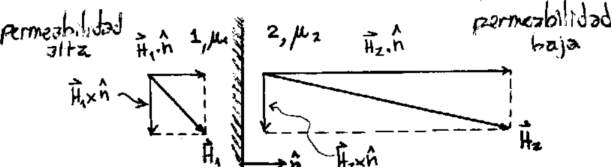
\includegraphics[width=0.4\textwidth]{images/fig_ft1_medios1.pdf}	 
	\end{center}
	\caption{}
\end{figure} 

\begin{figure}[htb]
	\begin{center}
	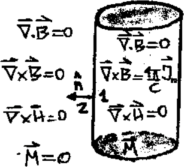
\includegraphics[width=0.4\textwidth]{images/fig_ft1_medios2.pdf}	 
	\end{center}
	\caption{}
\end{figure} 



\subsection{Teorema de Thomson}

\begin{figure}[htb]
	\begin{center}
	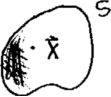
\includegraphics[width=0.4\textwidth]{images/fig_ft1_volume.pdf}	 
	\end{center}
	\caption{}
\end{figure} 


% =================================================================================================
\section{Magnetización}
% =================================================================================================

\begin{figure}[htb]
	\begin{center}
	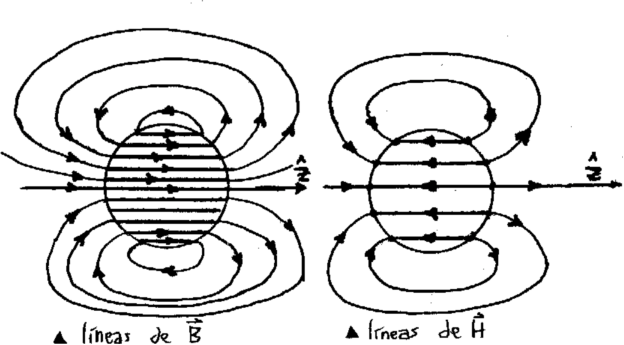
\includegraphics[width=0.4\textwidth]{images/fig_ft1_magnetiz1.pdf}	 
	\end{center}
	\caption{}
\end{figure} 

\begin{figure}[htb]
	\begin{center}
	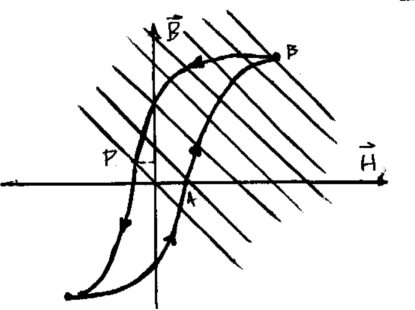
\includegraphics[width=0.4\textwidth]{images/fig_ft1_magnetiz2.pdf}	 
	\end{center}
	\caption{}
\end{figure} 

\begin{figure}[htb]
	\begin{center}
	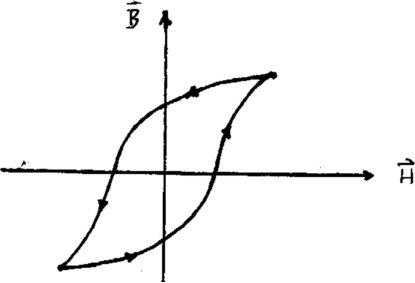
\includegraphics[width=0.4\textwidth]{images/fig_ft1_magnetiz3.pdf}	 
	\end{center}
	\caption{}
\end{figure} 

% =================================================================================================
\section{Tensor de Maxwell}
% =================================================================================================

\begin{figure}[htb]
	\begin{center}
	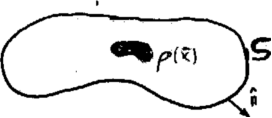
\includegraphics[width=0.4\textwidth]{images/fig_ft1_maxwell.pdf}	 
	\end{center}
	\caption{}
\end{figure} 

\subsection{Ejemplos del tensor de Maxwell}

\begin{figure}[htb]
	\begin{center}
	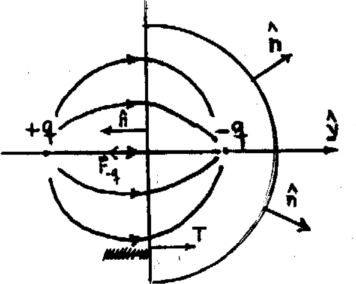
\includegraphics[width=0.4\textwidth]{images/fig_ft1_tensorM1.pdf}	 
	\end{center}
	\caption{}
\end{figure} 

\begin{figure}[htb]
	\begin{center}
	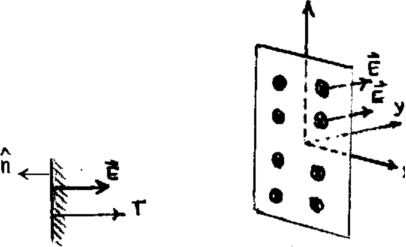
\includegraphics[width=0.4\textwidth]{images/fig_ft1_tensorM2.pdf}	 
	\end{center}
	\caption{}
\end{figure} 

\begin{figure}[htb]
	\begin{center}
	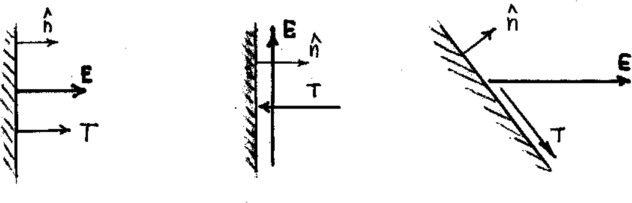
\includegraphics[width=0.4\textwidth]{images/fig_ft1_tensorM3.pdf}	 
	\end{center}
	\caption{}
\end{figure} 

\begin{figure}[htb]
	\begin{center}
	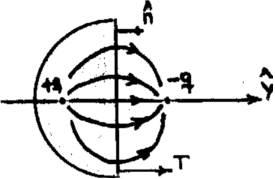
\includegraphics[width=0.4\textwidth]{images/fig_ft1_tensorM4.pdf}	 
	\end{center}
	\caption{}
\end{figure} 

\begin{figure}[htb]
	\begin{center}
	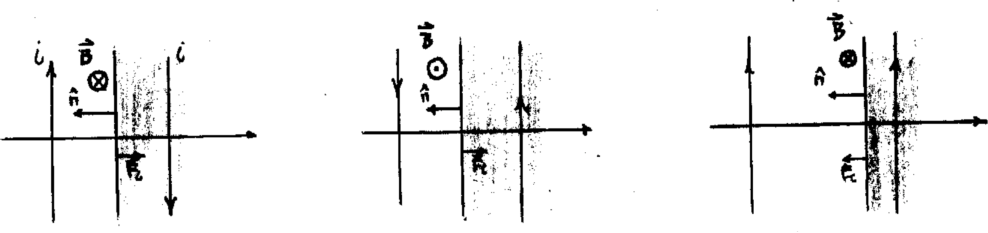
\includegraphics[width=0.4\textwidth]{images/fig_ft1_tensorM5.pdf}	 
	\end{center}
	\caption{}
\end{figure} 



% \bibliographystyle{CBFT-apa-good}	% (uses file "apa-good.bst")
% \bibliography{CBFT.Referencias} % La base de datos bibliográfica

\end{document}
